\section{Methodology}
\label{sec:method}
\begin{figure}[t]
\centering
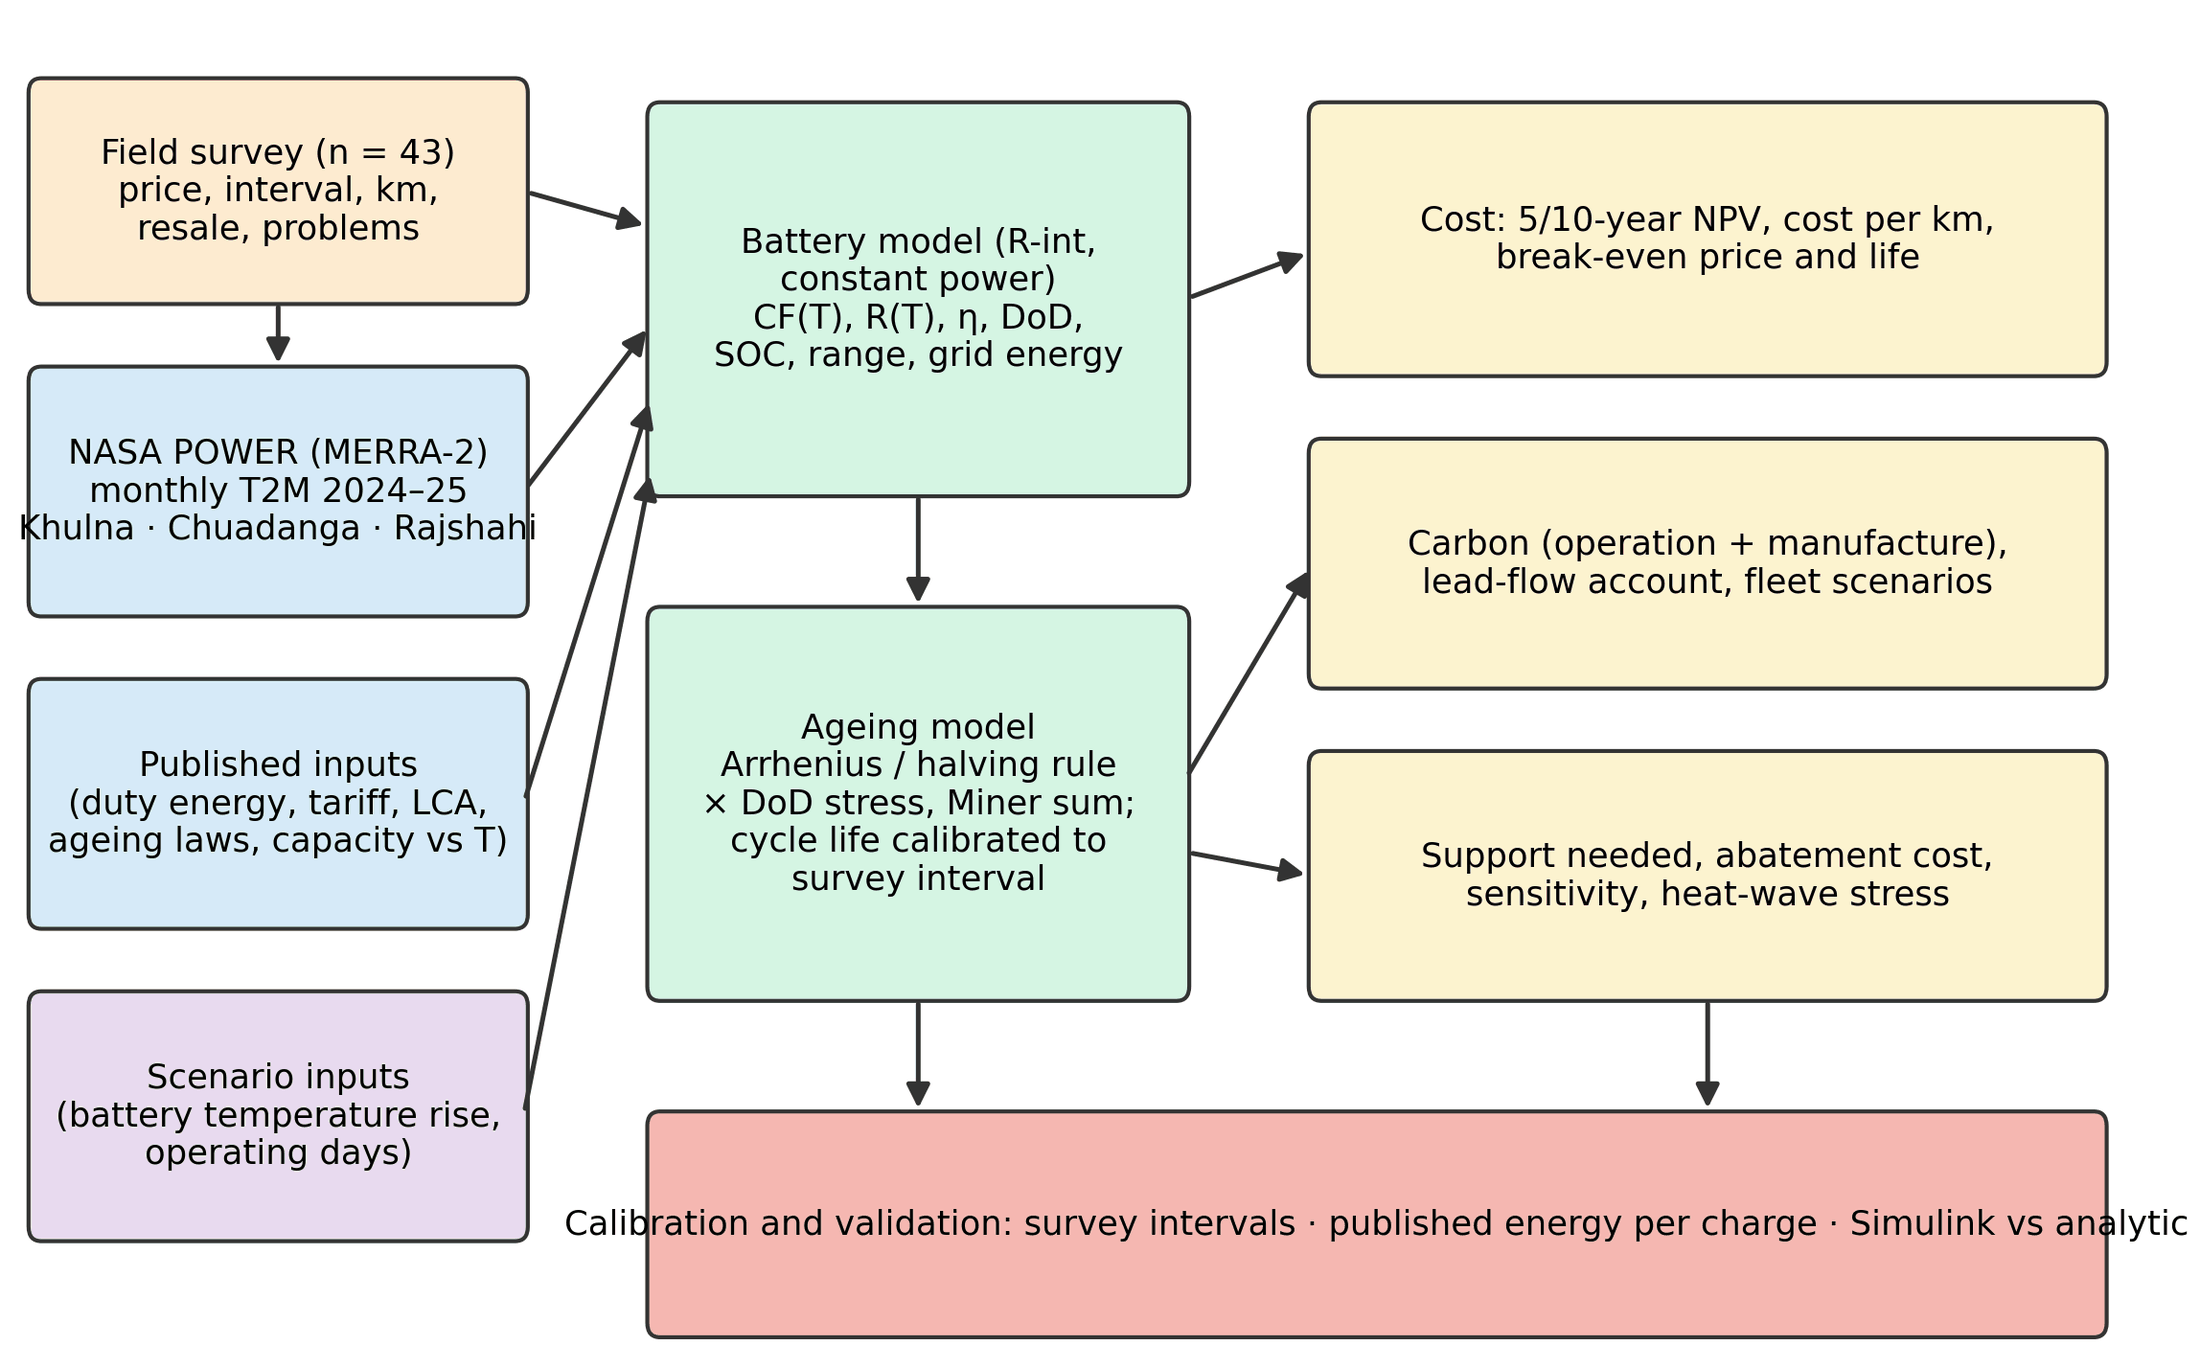
\includegraphics[width=\textwidth]{fig_method.png}
\caption{Methodology: survey, temperature, published and scenario inputs drive the battery and ageing models; outputs feed the cost, carbon, lead and policy modules; calibration and validation close the loop.}
\label{fig:method}
\end{figure}
\subsection{Study design and sites}
Three south-western sites are used for temperature: Khulna (22.84$^\circ$N, 89.57$^\circ$E), Chuadanga (23.64$^\circ$N, 88.69$^\circ$E) and Rajshahi (24.38$^\circ$N, 88.60$^\circ$E) (\figref{map}). The survey was carried out in the Khulna region (\todo{[insert district and upazila names]}), so Khulna is the calibration site; the other two sites are extrapolations through temperature only. Chuadanga was added as a heat-stress site because a 42\,$^\circ$C day was reported there in May 2025 \cite{heat2025}; in the NASA monthly means its annual mean in 2025 (\TannChuadangaBtwofive\,$^\circ$C) is not higher than Khulna's (\TannKhulnaBtwofive\,$^\circ$C), so its selection rests on peak heat, not on the mean. Two chemistries are modelled: lead-acid (LA) and LFP, the only lithium type reported in the survey.
\begin{figure}[t]
\centering
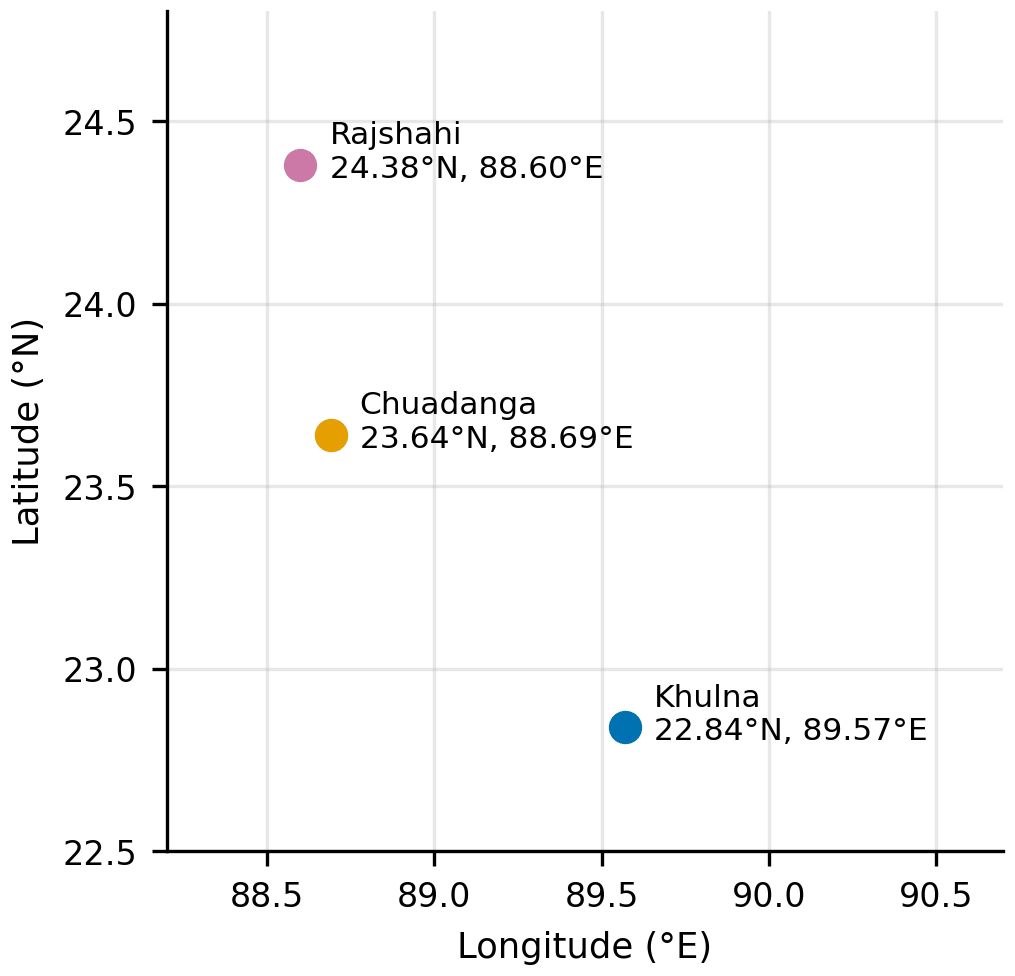
\includegraphics[width=0.5\textwidth]{fig_map.png}
\caption{NASA POWER grid points used (schematic locator).}
\label{fig:map}
\end{figure}

\subsection{Field survey}
\label{sec:survey}
Data come from a Bengali-language Google Forms questionnaire, ``Field Survey on Easy-Bike/E-Rickshaw Battery Use in Bangladesh'' \cite{survey2026}, with ten questions covering battery type, purchase cost, battery configuration, daily distance, charging frequency and cost, months in use, replacement interval, main problem and resale value. It recorded \nSurvey{} responses between 8 and 28 October 2026 from current drivers. The sample is a convenience sample, so the results are descriptive. \todo{[State ethical approval or consent procedure, and the survey locations.]}

Raw answers mixed Bengali and Western digits, ``k'' suffixes, ranges and units. Each field was converted to one unit; ``k'' was read as thousands of taka, ranges were represented by their mid-points, and the original sheet was kept unchanged. Interpreted values were flagged in a review-notes column (Appendix~\ref{app:survey}). Table~\ref{tab:use} shows which survey fields enter the model and which were deliberately not used.
\begin{table}[t]
\caption{Use of survey data in the model.}
\label{tab:use}
\centering\footnotesize
\renewcommand{\arraystretch}{1.1}
\begin{tabular}{p{3.6cm}p{5.0cm}p{6.0cm}}
\hline
Survey field & Use & Note \\
\hline
Purchase cost of current set & Initial and replacement cost $C_0$ (median by type) & LA: \nLA{}; LFP: \nLFP{} respondents; seven lead-based entries of BDT 60{,}000 or more are flagged and handled by using medians \\
Replacement interval & Calibrates $N_{80}$ (Khulna) and validates the model & LA $n$ = \replNLA{}; LFP $n$ = \replNLFP{}; LFP answers are expectations because the sets are on average \ageMeanLFP{} months old \\
Daily distance & Duty $d$ & Mean of all respondents \\
Resale value of old set & Scrap fraction $s$ & Median resale/purchase ratio by type \\
Batteries per set; Ah per battery & Pack voltage and capacity & Ah reported by only four lead-acid respondents \\
Charges per day & $n_{cyc}$ = 1 & \onePerDay{} of \nSurvey{} charge once \\
Main problem; months in use & Qualitative check of ageing-limited life & Not a model input \\
Charging cost & \emph{Not used} & Answers mix per-charge, per-month and unspecified bases and are not comparable \\
``Powder'' batteries & \emph{Not modelled} & Chemistry not confirmed; reported separately (\nPW{} respondents) \\
\hline
\end{tabular}
\end{table}

\subsection{Temperature data}
Monthly mean 2\,m air temperature (T2M, MERRA-2 \cite{gelaro2017}) for January 2024 to December 2025 was downloaded from NASA POWER \cite{nasa_power}: 24 values per site, none missing. The native grid cell is $0.5^\circ\times0.625^\circ$ (about 50--70 km), so the three points lie in neighbouring cells and are expected to be similar. Battery temperature is ambient plus $\Delta T_{op}=5\,^\circ$C, a scenario tested at 0 and 10\,$^\circ$C. Monthly means understate daily peaks (Section~\ref{sec:limits}).

\subsection{Battery model}
Each pack is a resistive (R-int) battery with temperature-dependent capacity and resistance, discharged at constant average power $P_w=e_{km}v$, where $e_{km}$ is the energy use per km and $v$ the average speed. With pack voltage $V$ and round-trip efficiency $\eta_{RT}$, the 25\,$^\circ$C resistance is chosen so that the discharge efficiency equals $\sqrt{\eta_{RT}}$ at 25\,$^\circ$C:
\begin{align}
R_{25}&=\frac{(1-\sqrt{\eta_{RT}})\sqrt{\eta_{RT}}\,V^{2}}{P_w},\\
R(T)&=R_{25}\exp\!\left[\frac{E_r}{R_g}\!\left(\frac1{T_K}-\frac1{298.15}\right)\right],\\
I&=\frac{V-\sqrt{V^{2}-4R(T)P_w}}{2R(T)},\qquad
\eta_d=1-\frac{I\,R(T)}{V}.
\end{align}
The capacity factor $CF(T)$ is interpolated from a table, so the available energy is $E_{cap}=V\,Ah\,CF(T)/1000$ kWh. With daily delivered energy $E_{day}=d\,e_{km}/1000$ for distance $d$,
\begin{align}
\mathrm{DoD}&=\frac{E_{day}}{\eta_d\,E_{cap}},\qquad
\mathrm{SOC}_{end}=\max(0,1-\mathrm{DoD}),\\
E_{grid}&=\frac{E_{day}}{\eta_d^{2}\,\eta_{chg}},\qquad
\mathrm{Range}=\frac{\mathrm{DoD}_{max}\,E_{cap}\,\eta_d}{e_{km}/1000}.
\end{align}
The same equations are implemented as a Simulink model built from core blocks (\figref{simulink}). It is run at 15, 25, 35 and 45\,$^\circ$C for both chemistries and compared with the analytic code (Appendix~\ref{app:sim}).
\begin{figure}[t]
\centering
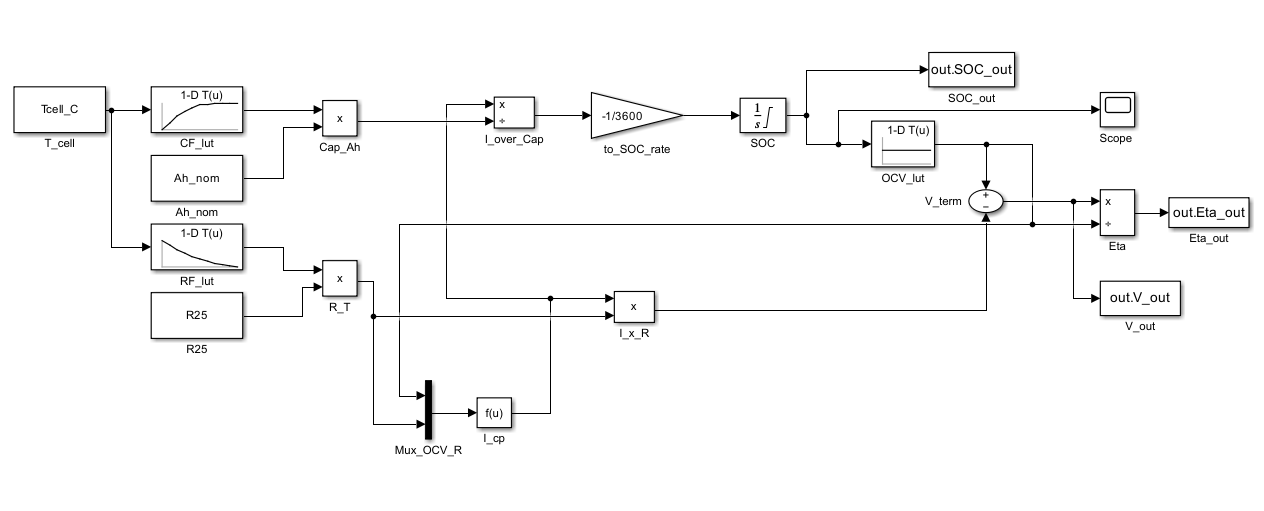
\includegraphics[width=\textwidth]{fig_simulink.png}
\caption{Block diagram of the Simulink model \texttt{easybike\_battery.slx}: temperature drives the capacity and resistance lookup tables; a function block solves the constant-power current; the integrator gives SOC.}
\label{fig:simulink}
\end{figure}

\subsection{Degradation, calibration and lifetime}
Cycle life falls with depth of discharge and temperature, and damage is accumulated month by month with Miner's rule \cite{miner1945}, as also done for variable-temperature VRLA service \cite{tsujikawa2009}:
\begin{align}
N_{eff,m}&=N_{80}\left(\frac{0.8}{\max(\mathrm{DoD}_m,0.05)}\right)^{k} f_T(T_m),\\
D&=n_{cyc}\sum_m \frac{w_m}{N_{eff,m}},\qquad L=\frac{1}{D\,d_{op}}\ \text{(years)},
\end{align}
where $w_m$ is the day-weighted share of month $m$, $d_{op}=300$ operating days per year and $n_{cyc}=1$. For LFP, $f_T=\min\{1,\exp[\tfrac{E_a}{R_g}(\tfrac1{T_K}-\tfrac1{298.15})]\}$ with $E_a=37.3$ kJ/mol \cite{yagci2026}; for lead-acid, $f_T=\min\{1,2^{-(T-25)/8}\}$ \cite{bu806a}. There is no life credit below 25\,$^\circ$C, and calendar ageing is not modelled.

The cycle life at 80\% DoD, $N_{80}$, is the least certain input: literature ranges (400 and 2{,}500 cycles) come from stationary storage. We therefore fit $N_{80}$ for each chemistry so that the modelled life at Khulna equals the survey median replacement interval. Because $N_{eff}$ is proportional to $N_{80}$ the fit is exact and unique. The fitted value is an \emph{effective field cycle life}: it also absorbs the unknown number of operating days, charging practice and battery quality. Calibration uses the Khulna temperature series only; the other two sites then follow from temperature alone. Before calibration the model is run with the literature values and compared with the survey (Section~\ref{sec:valid}); this comparison is the main validation.

\subsection{Total cost of ownership}
The 5- and 10-year net present cost with discount rate $r$ is
\begin{equation}
\mathrm{TCO}_H=C_0+\sum_{j=1}^{K}\frac{C_0(1-s)}{(1+r)^{jL}}-\frac{C_0\,\rho_H}{(1+r)^{H}}+\sum_{t=1}^{H}\frac{E_{grid}\,d_{op}\,\tau + m\,C_0}{(1+r)^t},
\end{equation}
with $C_0$ the set price, $K=\lfloor H/L\rfloor$ replacements, $s$ the resale fraction, $\rho_H$ the residual life fraction at horizon $H$, $\tau$ the tariff and $m$ the maintenance fraction. Cost per km is $\mathrm{TCO}_{10}$ divided by the discounted distance. Only battery-related cost is counted. Break-even set price and life are found by bisection on $\mathrm{TCO}_{10}(\mathrm{LFP})=\mathrm{TCO}_{10}(\mathrm{LA})$.

\subsection{Carbon, lead and policy}
Annual emissions per bike are $E_{CO_2}=E_{grid}\,d_{op}\,EF_{grid}+\varepsilon\,Q_{nom}\,12/L_{mo}$, with $EF_{grid}=0.62$ tCO$_2$/MWh \cite{doe_gef}, $Q_{nom}$ the pack energy, $L_{mo}$ the life in months and $\varepsilon=40$ and 50 kg CO$_2$e/kWh for LA and LFP \cite{jasper2025}. LFP packs are imported, so $\varepsilon$ is tested up to 110. Informal-smelting emissions have no verified factor and are excluded, which biases the lead-acid footprint downward. Lead cycled per year is $M_{Pb}=N\,m_{Pb}\,12/L_{mo}$ with $m_{Pb}$ = 56, 84 and 125 kg per lead-acid set: a mass flow, not an emission or a dose. Conversion scenarios move 0, 25, 50 and 100\% of a 1.4 M fleet from LA to LFP; outputs scale linearly. The \emph{operator support} needed is the 10-year cost gap per bike times the number converted, and the implied abatement cost is that gap divided by ten years of CO$_2$e saved. These quantities are indicative: they ignore health benefits, taxes and import costs.

\subsection{Validation and sensitivity}
Checks are: V1 data integrity (24 monthly values per site, none missing); V2 model life against survey replacement intervals, before and after calibration; V3 grid energy per bike-day against the 8--9 kWh per charge of the field study \cite{chowdhury2026} and the CLEAN and UNCTAD fleet figures \cite{clean2024,unctad_smep} (not used for calibration, so independent); V4 Simulink against the analytic model; V5 consistency of the survey's range complaints with ageing-limited life. One-at-a-time sensitivity over eleven inputs (\figref{tornado}) uses ranges taken from the survey wherever it supplies one.
